\section{Evolúciós játékok}

\subsection{Klasszikus játékelméleti fogalmak}
\begin{frame}
\frametitle{Klasszikus játékelméleti fogalmak}
\begin{columns}[T]
	\begin{column}{0.5\linewidth}
\begin{itemize}
	\item játék
	\item játékosok
	\item szabályok
	\item nyereség maximalizálása
\end{itemize}

	\end{column}

	\begin{column}{0.5\linewidth}
\begin{figure}
	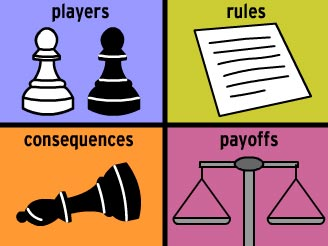
\includegraphics[width=\linewidth]{images/game-theory}
\end{figure}
	\end{column}
\end{columns}

\end{frame}


\subsection{Játékelmélet a biológiában}
\begin{frame}
\frametitle{Játékelmélet a biológiában}
\begin{itemize}
	\item játékelmélet alkalmazása a populációk alakulásának vizsgálatára
	\item játékosok - nem racionálisak
	\item fitnesz mint nyereség
	\item evolúciósan stabil stratégia - az azt alkalmazó populáció nem győzhető le semmilyen más, kezdetben kevés létszámú stratégiával
\end{itemize}
\end{frame}
